\documentclass[dvisvgm,border=8pt]{standalone}
\usepackage{amsmath,amssymb}
\usepackage[scaled]{helvet}\renewcommand{\familydefault}{\sfdefault}
\usepackage{tikz}\usetikzlibrary{positioning,arrows.meta,calc}
\definecolor{gin}{HTML}{F5F5F5}\definecolor{gstroke}{HTML}{666666}
\definecolor{dg}{HTML}{6D8764}\definecolor{dgs}{HTML}{3A5431}
\definecolor{exg}{HTML}{2E7D32}\definecolor{warn}{HTML}{B46504}
\newcommand{\ex}[1]{\textcolor{exg}{#1}}
\tikzset{font=\small, >={Stealth[length=2.2mm]},
  base/.style={draw, rounded corners=3pt, align=center, inner sep=5pt, minimum height=9mm},
  inp/.style={base, fill=gin, draw=gstroke},
  calc/.style={base, fill=white, draw=black},
  res/.style={base, fill=dg, draw=dgs, text=white},
  ar/.style={->, thick}}
\begin{document}
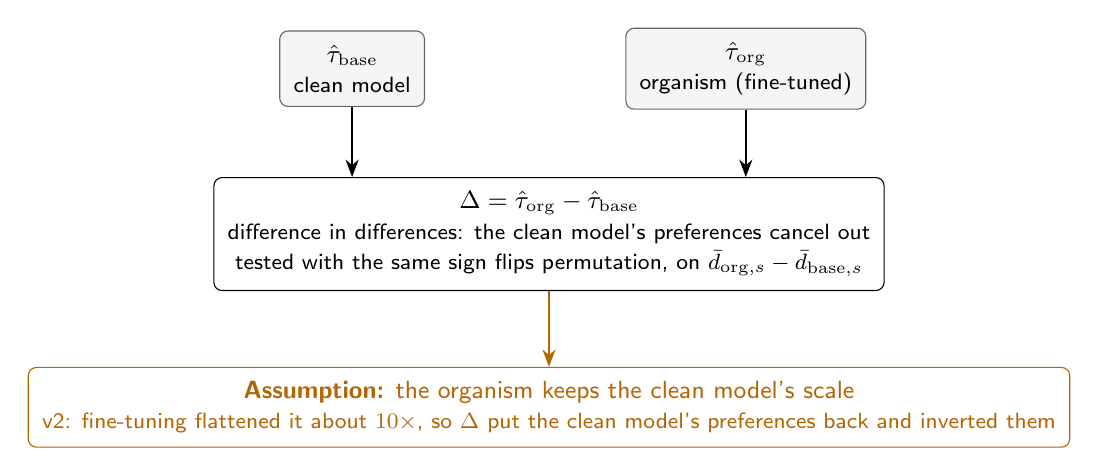
\begin{tikzpicture}
\node[inp] (B) at (0,0) {$\hat\tau_{\mathrm{base}}$\\{\footnotesize clean model}};
\node[inp] (O) at (5,0) {$\hat\tau_{\mathrm{org}}$\\{\footnotesize organism (fine-tuned)}};
\node[calc] (D) at (2.5,-2.1) {$\Delta=\hat\tau_{\mathrm{org}}-\hat\tau_{\mathrm{base}}$\\{\footnotesize difference in differences: the clean model's preferences cancel out}\\{\footnotesize tested with the same sign flips permutation, on $\bar d_{\mathrm{org},s}-\bar d_{\mathrm{base},s}$}};
\node[base, draw=warn, text=warn, fill=white] (A) at (2.5,-4.3) {\textbf{Assumption:} the organism keeps the clean model's scale\\{\footnotesize v2: fine-tuning flattened it about $10\times$, so $\Delta$ put the clean model's preferences back and inverted them}};
\draw[ar] (B.south) -- (B.south |- D.north); \draw[ar] (O.south) -- (O.south |- D.north); \draw[ar, draw=warn] (D) -- (A);
\end{tikzpicture}
\end{document}
